\section{Modelo transaccional}
\label{TransactionalModel}

	Para mostrar el funcionamiento del aspecto transaccional, utilizaremos como
	ejemplo un Producto. El producto tiene un stock y un state, que especifica si
	el producto está habilitado o deshabilitado para la venta. 
	
	La Figura \ref{transactionalModel} muestra esquemáticamente como se ve el
	los contextos transaccionales a medida que el objeto recibe mensajes de
	modificación.

	\begin{figure}
		\begin{tabular}{cc}
		\centering
			\subfloat[Se crean dos transacciones simultaneas]{
	    		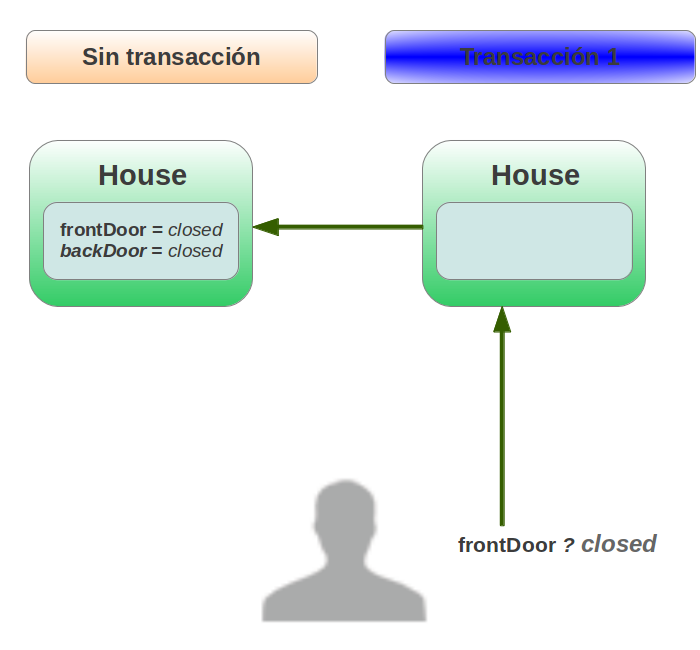
\includegraphics[scale=0.4]{img/contextoAninado1}
	    	}&
			\subfloat[Dentro del primer contexto se modifica el stock del producto, y
			ese cambio no es visible para el segundo contexto.]{
	    		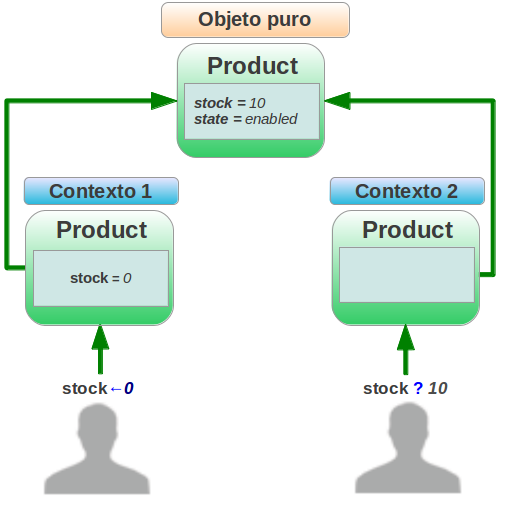
\includegraphics[scale=0.4]{img/contextoAninado2}
	    	}\\
			\subfloat[Dentro del segundo contexto se modifica el estado del producto, y
			ese cambio no es visible para el primer contexto.]{
	    		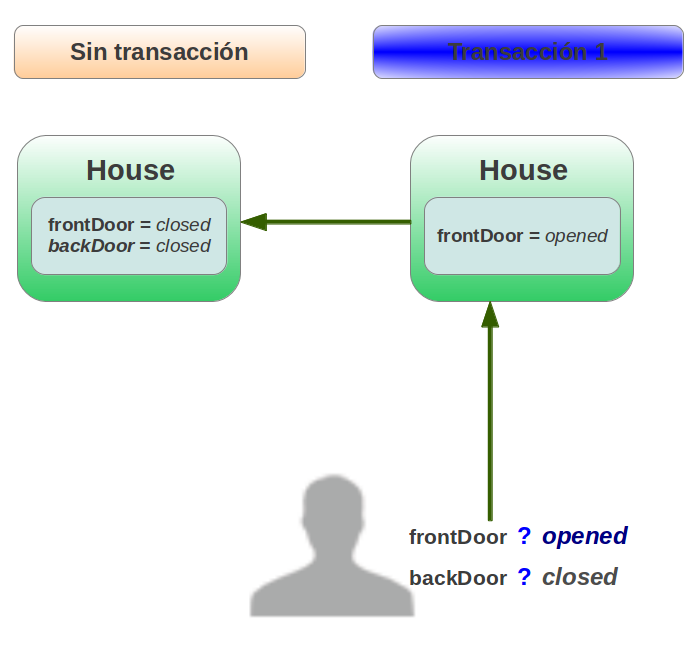
\includegraphics[scale=0.4]{img/contextoAninado3}
	    	}&
			\subfloat[El primer contexto realiza un commit confirmando sus cambios e
			impactando los mismos en el objeto; el segundo contexto se entera de esa
			modificación.]{
	    		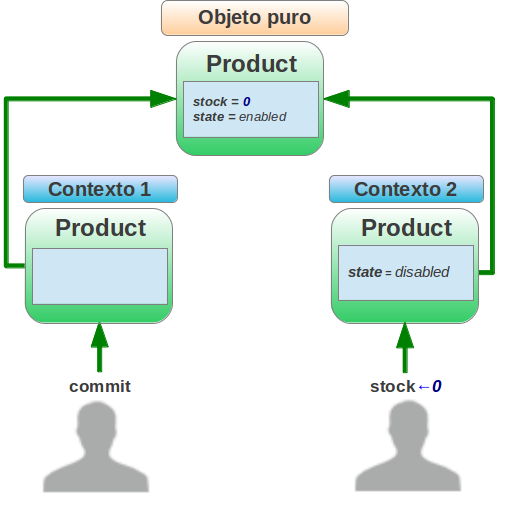
\includegraphics[scale=0.4]{img/contextoAninado4}
	    	}\\
			\subfloat[Se crea una nueva transacción anidada a la segunda.]{
	    		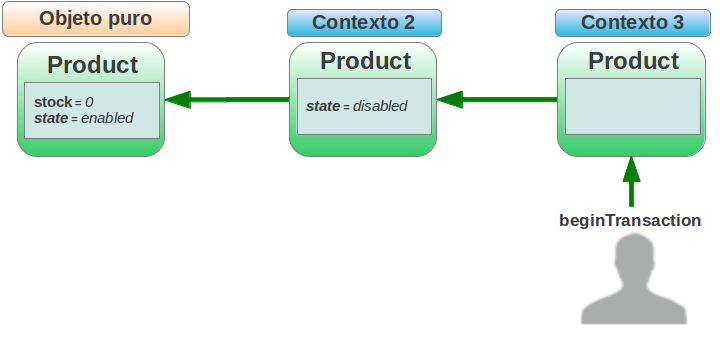
\includegraphics[scale=0.35]{img/contextoAninado5}
			}&
			\subfloat[Los cambios mutuos no son visibles fuera de su contexto.]{
	    		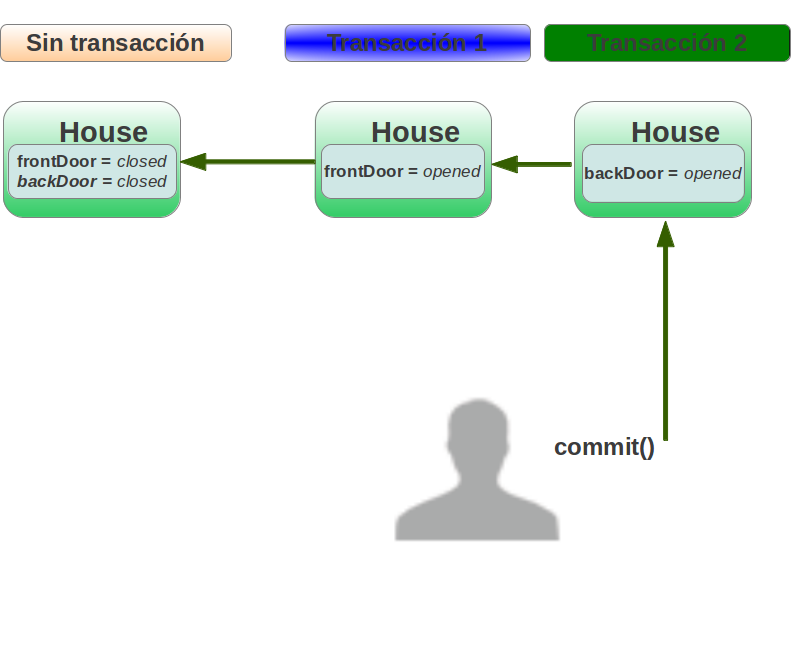
\includegraphics[scale=0.35]{img/contextoAninado6}
	    	}\\
			\subfloat[La transacción confirma sus cambios y estos son impactados
			en la transacción padre]{
	    		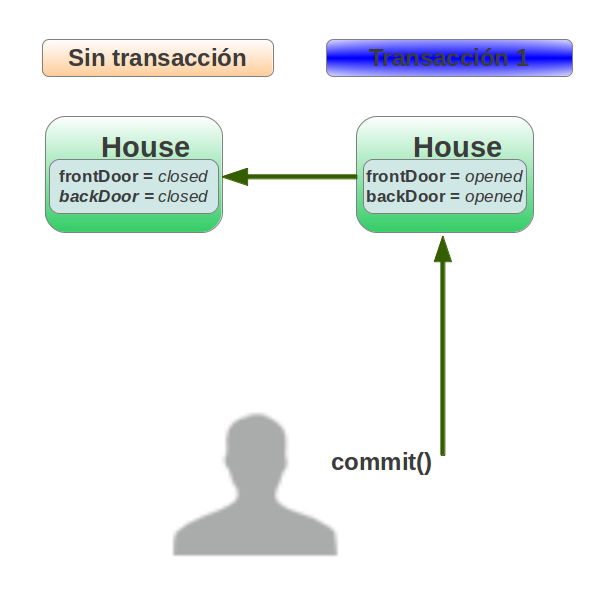
\includegraphics[scale=0.35]{img/contextoAninado7}
	    	}&
			\subfloat[La última transacción realiza un commit, y todos los cambios con
			impactados en el objeto.]{
	    		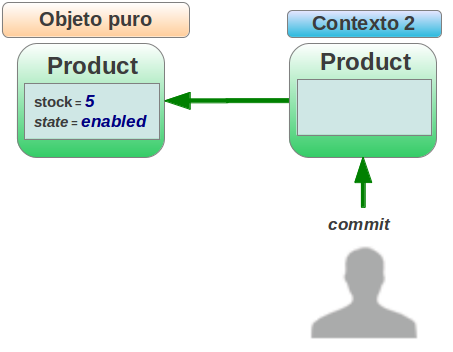
\includegraphics[scale=0.4]{img/contextoAninado8}
	    	}
			\end{tabular}
		\caption{Ejemplo del modelo transaccional}
		\label{transactionalModel}
	\end{figure}
